\section{Test data generation}

In this section we present the algorithm that generates test data
from a model written in the modeling language defined in
Section~\ref{sec:model}. 

At its core the algorithm uses backwards substitution to generate a
sequence of operations that puts the application into the desired
state needed to cover a given a target operation. 

\subsection{Control Flow Graph Representation of Models}
\label{sec:control-flow-graph}

Before the actual backwards substitution takes place the model is
converted into a control flow graph(CFG) representation. The process of
converting a single operation to it's CFG is
illustrated in Figure~\ref{fig:cfg}. As the preconditions of all rules in
a group are disjoint, control flow through a single group can cover
exactly one precondition-post condition pair. The CFG reflects this by
representing a single group as a choice between the available rules, as
seen in Figure~\ref{fig:cfgb}. Given a CFG component for each group in
the operation, we model the entire operation by sequencing all
components (Figure~\ref{fig:cfgc}). As per well-formedness property 4
there is data dependence between rules in an operation and therefore
all orderings are equivalent.

\begin{figure*}
%  \centering
  \begin{subfigure}[b]{0.4\textwidth}
    \centering
    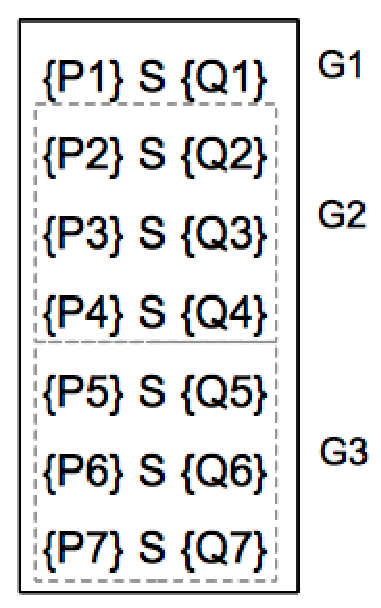
\includegraphics[width=.4\linewidth]{figs/cfg-example1}
    \caption{An operation}
    \label{fig:cfga}
  \end{subfigure}%
  \begin{subfigure}[b]{0.4\textwidth}
    \centering
    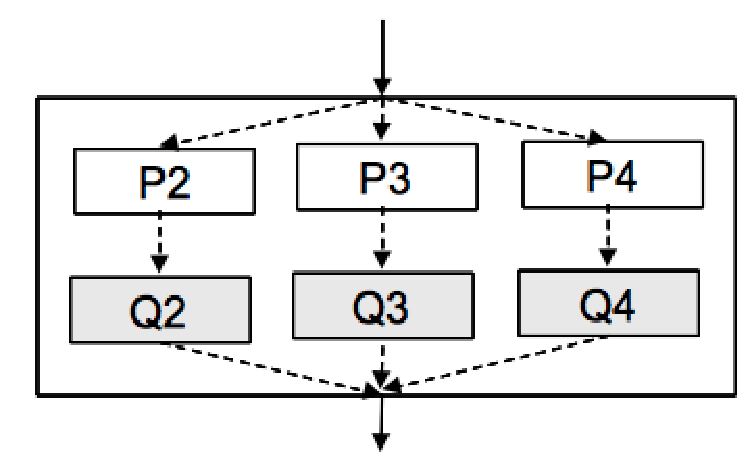
\includegraphics[width=.4\linewidth]{figs/cfg-example2}
    \caption{The interopertational flow for group 2}
    \label{fig:cfgb}
  \end{subfigure}%
  \begin{subfigure}[b]{0.2\textwidth}
    \centering
    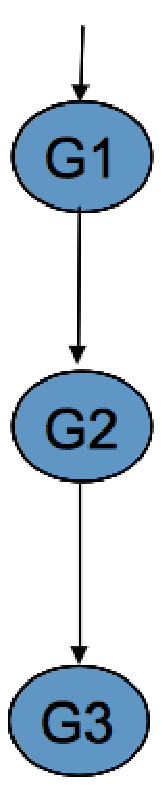
\includegraphics[width=.4\linewidth]{figs/cfg-example3}
    \caption{The CFG component for the entire operation}
    \label{fig:cfgc}
  \end{subfigure}%
  \caption{Control flow graph generation for a single operation}
  \label{fig:cfg}
\end{figure*}

The interoperational flow is defined by the input/output relations
between operations. An operation creating an entity will naturally be
succeeded by any operation modifying the entity. These edges can either
be setup initially or created on demand during backwards substitution. 

Some edges are specified directly by the designer of the model...next
and triggers

\subsection{Binding}
\label{sec:binding}

When sequencing two operations we need to substitute the entities
consumed by the successor operation by the entities created or
modified by the predecessor operation.

In our algorithm we move this problem to the underlying constraint
solver by creating constraints that bind the identifiers in the post
condition of the predecessor operation to the identifiers of same type
in the pre condition of the successor operation. As the solver has no
notion of objects, the binding must also ensure that object fields
referenced are appropriately bound.

Binding constraints are generated as follows: Assume that we want to
sequence the two operations $O_{pred}$ and $O_{succ}$ and that the
algorithm have chosen rules $r_1$ and $r_2$ from $O_{pred}$ and
$O_{succ}$ respectively for the sequencing. Now let $v$ be an
identifer of type $\tau$ occuring in either the creates or modfies
clause of $O_{pred}$ and let $w$ be an identifier of same type
occuring in the input clause of $O_{succ}$. If $\tau$ is an enum type,
the only binding needed is $w = v$. If $\tau$ is an object type, then
we must bind all subfields as well, yielding the following constraint:
$w = v \wedge w.f_1 = v.f_1 \wedge \ldots \wedge w.f_n = v.f_n$ where
$f_1, \ldots , f_n$ are fields declared on $\tau$. If any of the
fields are of object types themselves this process is applied
recursively on each such field to generate the final binding
constraint.

As an example of this process take the \emph{Compute Invoice Total}
operation shown in Figure~\ref{fig:invoice}... Include figure from
slide 12?
